\documentclass[12pt, a4paper, onecolumn, oneside, final]{report}

\usepackage{uithesis}

%-----------------------------------------------------------------------------%
% Informasi Mengenai Dokumen
%-----------------------------------------------------------------------------%
% 
\usepackage{booktabs}
\usepackage{bigstrut}

\usepackage{colortbl}
\usepackage{etoolbox}
\patchcmd{\tableofcontents}{\@starttoc}{\vspace{-1cm}\@starttoc}{}{}
%-----------------------------------------------------------------------------%
\setlength{\parindent}{0em}
\setlength{\parskip}{1em}

% Judul laporan. 
\var{\judul}{DESAIN DAN SIMULASI
	PERLINDUNGAN PROPERTI INTELEKTUAL
	MENGGUNAKAN ALGORITME FILTER DIGITAL}
% 
% Tulis kembali judul laporan, kali ini akan diubah menjadi huruf kapital
\Var{\Judul}{DESAIN DAN SIMULASI
	PERLINDUNGAN PROPERTI INTELEKTUAL
	MENGGUNAKAN ALGORITME FILTER DIGITAL}
% 
% Tulis kembali judul laporan namun dengan bahasa Ingris
\var{\judulInggris}{DESIGN AND SIMULATION OF INTELECTUAL PROPERTIES PROTECTION
	USING DIGITAL FILTER ALGORITHM}

% 
% Tipe laporan, dapat berisi Skripsi, Tugas Akhir, Thesis, atau Disertasi
\var{\type}{Tugas Akhir}
% 
% Tulis kembali tipe laporan, kali ini akan diubah menjadi huruf kapital
\Var{\Type}{Tugas Akhir}
% 
% Tulis nama penulis 
\var{\penulis}{Hanjara Cahya Adhyatma}
% 
% Tulis kembali nama penulis, kali ini akan diubah menjadi huruf kapital
\Var{\Penulis}{Hanjara Cahya Adhyatma}
% 
% Tulis NPM penulis
\var{\npm}{1104131113}
% 
% Tuliskan Fakultas dimana penulis berada
\Var{\Fakultas}{Teknik Elektro}
\var{\fakultas}{Teknik Elektro}
% 
% Tuliskan Program Studi yang diambil penulis
\Var{\Program}{S1 Sistem Komputer}
\var{\program}{S1 Sistem Komputer}
% 
% Tuliskan tahun publikasi laporan
\Var{\bulanTahun}{2017}
% 
% Tuliskan gelar yang akan diperoleh dengan menyerahkan laporan ini
\var{\gelar}{S1 Sistem Komputer}
% 
% Tuliskan tanggal pengesahan laporan, waktu dimana laporan diserahkan ke 
% penguji/sekretariat
\var{\tanggalPengesahan}{XX Juli 2017} 
% 
% Tuliskan tanggal keputusan sidang dikeluarkan dan penulis dinyatakan 
% lulus/tidak lulus
\var{\tanggalLulus}{XX Januari 2010}
% 
% Tuliskan pembimbing 
\var{\pembimbing}{Prof. XXXX}
% 
% Alias untuk memudahkan alur penulisan paa saat menulis laporan
\var{\saya}{Penulis}

%-----------------------------------------------------------------------------%
% Judul Setiap Bab
%-----------------------------------------------------------------------------%
% 
% Berikut ada judul-judul setiap bab. 
% Silahkan diubah sesuai dengan kebutuhan. 
% 
\Var{\kataPengantar}{KATA PENGANTAR}
\Var{\babSatu}{Pendahuluan}
\Var{\babDua}{Tinjauan Pustaka}
\Var{\babTiga}{Desain dan Simulasi}
\Var{\babEmpat}{Pengujian dan Analisis}
\Var{\babLima}{Kesimpulan dan Saran}
\Var{\babEnam}{Apa Ya}
\Var{\kesimpulan}{Kesimpulan dan Saran}


\hyphenation{
    % alphabhet A
    a-na-li-sa a-tur 
    a-pli-ka-si 
    % alphabhet B
    ba-ngun-an 
    be-be-ra-pa 
    ber-ge-rak
    ber-ke-lan-jut-an 
    ber-pe-nga-ruh
    ber-kurang 
    % alphabhet C
    ca-ri
    current
    % alphabhet D
    di-sim-pan di-pim-pin de-ngan da-e-rah di-ba-ngun da-pat di-nya-ta-kan 
    di-sim-bol-kan di-pi-lih di-li-hat de-fi-ni-si
    % alphabhet E
    e-ner-gi eks-klu-sif
    % alphabhet F
    fa-si-li-tas
    % alphabhet G
    ga-bung-an ge-rak
    % alphabhet H
    ha-lang-an
    % alphabhet I
    % alphabhet J
    % alphabhet K
    karena-nya
    ke-hi-lang-an
    ku-ning 
    kua-li-tas 
    ka-me-ra 
    ke-mung-kin-an 
    ke-se-pa-ham-an
    ke-rugian
    % alphabhet L
    ling-kung-an
    % alphabhet M
    me-neng-ah
    meng-a-tas-i me-mung-kin-kan me-nge-na-i me-ngi-rim-kan 
    meng-u-bah meng-a-dap-ta-si me-nya-ta-kan mo-di-fi-ka-si
    meng-a-tur
    % alphabhet N
    nya-ta non-eks-klu-sif
    % alphabhet O
    % alphabhet P
    pe-neliti-an
	pe-nye-rap-an 
	pe-ngon-trol
    pe-mo-del-an
    pe-ran  pe-ran-an-nya
    pem-ba-ngun-an pre-si-den pe-me-rin-tah prio-ri-tas peng-am-bil-an 
    peng-ga-bung-an pe-nga-was-an pe-ngem-bang-an 
    pe-nga-ruh pa-ra-lel-is-me per-hi-tung-an per-ma-sa-lah-an 
    pen-ca-ri-an peng-struk-tur-an
    % alphabhet Q
    % alphabhet R
    ran-cang-an
    % alphabhet S
    si-mu-la-si sa-ngat
    % alphabhet T
    te-ngah
    ter-da-pat
    % alphabhet U
    % alphabhet V
    % alphabhet W
    % alphabhet X
    % alphabhet Y
    % alphabhet Z
    % special
}

\var{\license}{\f{Creative Common License 1.0 Generic}}
\var{\bslash}{$\setminus$}

\begin{document}

\begin{titlepage}
    \begin{center}
    \vspace*{1.0cm}
    
    % judul thesis harus dalam 14pt Times New Roman
    \bo{\Judul} \\[1.0cm]
    \bo{\f{\Judulen}} \\[1.0cm]
    
    % harus dalam 14pt Times New Roman
    \bo{\Type} \\[1.0cm]
    
    % keterangan prasyarat
    \bo{Disusun sebagai syarat untuk memperoleh gelar \gelar \\ pada Program Studi \program\\ Universitas Telkom}\\[1.0cm]
    \bo{oleh}\\[1.0cm]
    
    % penulis dan npm
    \bo{\Penulis} \\
    \bo{\npm} \\
    \begin{figure}
    \begin{center}
    
\includegraphics[width=5.0cm]{pics/telu.png}
    \end{center}
    \end{figure}    
    
    % informasi mengenai fakultas dan program studi
    \bo{FAKULTAS \Fakultas\\UNIVERSITAS TELKOM\\BANDUNG \\\Tahun}
    \end{center}
\end{titlepage}


\pagenumbering{roman}

\addChapter{HALAMAN JUDUL}
\begin{titlepage}
    \begin{center}
    \vspace*{1.0cm}
    
    % judul thesis harus dalam 14pt Times New Roman
    \bo{\Judul} \\[1.0cm]
    \bo{\f{\Judulen}} \\[1.0cm]
    
    % harus dalam 14pt Times New Roman
    \bo{\Type} \\[1.0cm]
    
    % keterangan prasyarat
    \bo{Disusun sebagai syarat untuk memperoleh gelar \gelar \\ pada Program Studi \program\\ Universitas Telkom}\\[1.0cm]
    \bo{oleh}\\[1.0cm]
    
    % penulis dan npm
    \bo{\Penulis} \\
    \bo{\npm} \\
    \begin{figure}
    \begin{center}
    
\includegraphics[width=5.0cm]{pics/telu.png}
    \end{center}
    \end{figure}    
    
    % informasi mengenai fakultas dan program studi
    \bo{FAKULTAS \Fakultas\\UNIVERSITAS TELKOM\\BANDUNG \\\Tahun}
    \end{center}
\end{titlepage}


\setcounter{page}{2}

\addChapter{LEMBAR PENGESAHAN}
%
% Halaman Pengesahan
%
% @author  Andreas Febrian
% @version 1.01
%

\chapter*{HALAMAN PERSETUJUAN}

\vspace*{0.2cm}
\noindent 

\noindent
\begin{tabular}{l l p{11cm}}
	\bo{Judul}&: & \judul \\ 
	\bo{Nama}&: & \penulis \\
	\bo{NPM}&: & \npm \\
\end{tabular} \\

\vspace*{1.2cm}

\noindent Laporan \type~ini telah diperiksa dan disetujui.\\[0.3cm]
\begin{center}
\tanggalPengesahan \\[2cm]


\underline{\pembimbing}\\[0.1cm]
Pembimbing \type
\end{center}

\newpage

\addChapter{LEMBAR PERNYATAAN ORISINALITAS}
\chapter*{\uppercase{halaman pernyataan orisinalitas}}

\vspace*{0.4cm}
\noindent 

\noindent
\begin{tabular}{ll p{10cm}}
	NAMA&: & \penulis \\
	NIM&: & \nim \\
	ALAMAT&: & \alamat \\
	No. TLP/HP&: & \tlp \\
	E-MAIL&: & \email \\
\end{tabular} \\

\vspace*{1.0cm}

\noindent Menyatakan bahwa Tugas Akhir II ini merupakan karya orisinal saya sendiri dengan judul:\\
\begin{center}
	\textbf{\judul}\\[0.5cm]
	\textit{\Judulen}\\[1.0cm]
\end{center}
\noindent Atas pernyataan ini, saya siap menanggung resiko/sanksi yang dijatuhkan kepada saya apabila kemudian ditemukan adanya pelanggaran terhadap kejujuran akademik atau etika keilmuan dalam karya ini, atau ditemukan bukti yang menunjukkan ketidak aslian karya ini.\\



\newpage

\addChapter{ABSTRAK}
\chapter*{Abstrak}

\noindent \textit{System on a Chip} (SoC) adalah sebuah modul \textit{embedded system} yang
memiliki fungsi tertentu dalam sebuah papan \textit{chip silicon} yang juga bisa disebut
dengan \textit{Veri Large Scale Integration} (VLSI). Pemilik dari desain SoC memiliki
hak cipta atas desain sistem yang telah dibuat. \textit{Fabless} manufacturing merupakan
cara pencetakan modul perangkat keras yang desainer \textit{Integrated Circuit} (IC)
adalah \textit{Outsourching} dari luar pabrik percetakan.

\vspace*{0.5cm}
\noindent \textit{Fabless} manufacturing dari desain IC memiliki celah pencurian desain
ketika desain akan dicetak atau ketika proyek membutuhkan \textit{mutiple module}
dengan berbagai fungsi dari berbagai desainer. Oleh karena itu setiap modul VLSI
dari desainer chip ini membutuhkan bukti \textit{ownership} dari perancang atau
perusahaan produksi. Dalam penelitian ini dibuat verifikasi \textit{ownership}
dengan 2 kunci khusus verifikasi yaitu \textit{Polygate} sebagai kunci utama yang akan
mengaktifkan kunci kedua, dan kunci kedua akan aktif yang prosesnya
menggunakan algoritme filter digital.

\vspace*{0.5cm}
\noindent Pengamanan menggunakan algoritma pengecoh/pembingung (\textit{Obfuscation}) untuk melindungi rangkaian utama. Rangkaian utama disisipkan dengan rangkaian pelindung tanpa merubah dan mengganggu fungsi utama rangkaian. Teknik pengecohan dilakukan pada \textit{behavioral level} dan \textit{sinthesis level}. Pada hasil kompilasi desain sintesis (RTL) didapat rangkaian utama dan pelindung tercampur menjadi satu. Sehingga pada hasil akhir desain seakan tidak ada rangkaian lain selain rangkaian utama. Serta apabila rangkaian berhasil di gandakan (\textit{cloning}) maka rangkaian tersebut dapat diklaim dengan menggunakan alat kusus untuk mengaktifkan rangkaian pelindung.

\vspace*{0.5cm}

\noindent \textbf{Kata Kunci}: VLSI, \textit{Intelectual Property Protection}, \textit{Digital Signal Processing}, \textit{Polygate Watermark}.

\newpage

\addChapter{ABSTRACT}
\chapter*{ABSTRACT}

\noindent System on a Chip (SoC) is an embedded system module
Has a certain functionality in a silicon chip board that can also be called
With Veri Large Scale Integration (VLSI). The owner of the SoC design has
Copyright over the system design that has been created. Fabless manufacturing is
How to mold a hardware module that is designer Integrated Circuit (IC)
Is Outsourching from outside the printing factory.

\vspace*{0.5cm}
\noindent Fabless manufacturing from IC design has gap design theft
When the design will be printed or when the project requires mutiple module
With various functions from various designers. Therefore every module is VLSI
From this chip designer requires proof of ownership from the designer or
Production company.

\vspace*{0.5cm}
\noindent In this study plans to make a verification of ownership design
With 2 dedicated verification keys ie Polygate as the primary key going
Activate the second key, and the second key will be active which process
Using a digital filter algorithm.

\vspace*{0.2cm}

\noindent \textbf{Keywords}: VLSI, Intellectual Property Protection, Digital Signal Processing, Polygate Watermark.

\newpage

\addChapter{\kataPengantar}
%-----------------------------------------------------------------------------%
\chapter*{\kataPengantar}
%-----------------------------------------------------------------------------%
Template ini disediakan untuk orang-orang yang berencana menggunakan 
\latex~untuk membuat dokumen tugas akhirnya. 
Mengapa \latex? 
Ada banyak hal mengapa menggunakan \latex, diantaranya:

\begin{enumerate}
	\item \latex~membuat kita jadi lebih fokus terhadap isi dokumen, bukan 
		tampilan atau halaman. 
	\item \latex~memudahkan dalam penulisan persamaan matematis. 
	\item Adanya automatis dalam penomoran caption, bab, subbab, subsubbab, 
		referensi, dan rumus. 
	\item Adanya automatisasi dalam pembuatan daftar isi, daftar gambar, dan
		daftar tabel. 
	\item Adanya kemudahan dalam memberikan referensi dalam tulisan dengan 
		menggunakan label. Cara ini dapat meminimalkan kesalahan pemberian 
		referensi. 
\end{enumerate}

Template ini bebas digunakan dan 
didistribusikan sesuai dengan aturan \license, yang secara sederhana berisi: 

\begin{figure}
	\centering
	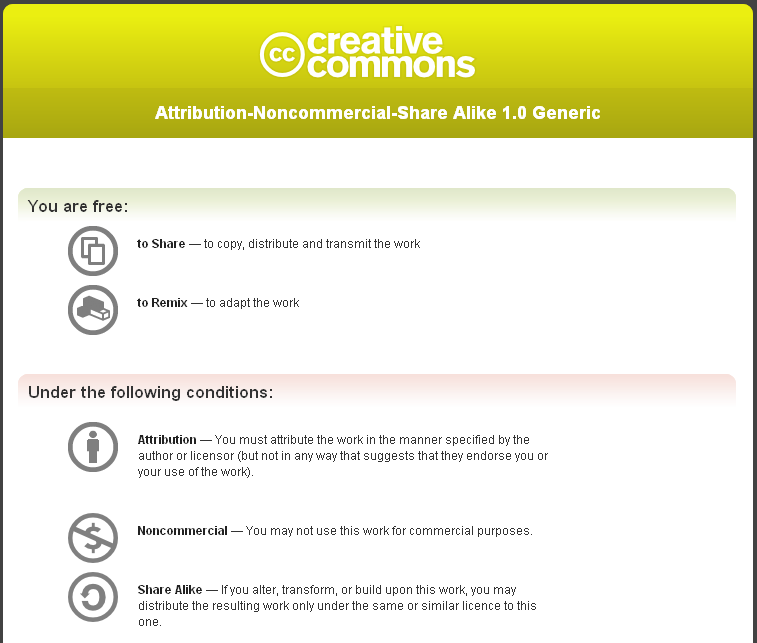
\includegraphics[width=0.74\textwidth]
		{pics/creative_common.png}
	\caption{\license}
	\label{fig:lisensi}
\end{figure}

\pic~\ref{fig:lisensi} diambil dari 
\url{http://creativecommons.org/licenses/by-nc-sa/1.0/deed.en_CA}. 
Jika ingin mengentahui lebih lengkap mengenai \license, silahkan buka 
\url{http://creativecommons.org/licenses/by-nc-sa/1.0/legalcode}. 
Seluruh dokumen yang dibuat dengan menggunakan template ini sepenuhnya 
menjadi hak milik pembuat dokumen dan bebas didistribusikan sesuai dengan 
keperluan masing-masing. 
Lisensi hanya berlaku jika ada orang yang membuat template baru dengan 
menggunakan template ini sebagai dasarnya. 

Dokumen ini dibuat dengan \latex~juga. Untuk meyakinkan Anda, coba lihat 
properti dari dokumen ini dan Anda akan menemukan bagian seperti 
\pic~\ref{fig:pdflatex}. 
Dokumen ini dimaksudkan untuk memberikan gambaran kepada Anda seperti apa 
mudahnya menggunakan \latex~dan juga memperlihatkan betapa bagus dokumen 
yang dihasilkan. 
Seluruh url yang Anda temukan dapat Anda klik. 
Seluruh referensi yang ada juga dapat diklik. 
Untuk mengerti template yang disediakan, Anda tetap harus membuka kode 
\latex~dan bermain-main dengannya. 
Penjelasan dalam PDF ini masih bersifat gambaran dan tidak begitu 
mendetail, dapat dianggap sebagai pengantar singkat. 
Jika Anda merasa kesulitan dengan template ini, mungkin ada baiknya 
Anda belajar sedikit dasar-dasar \latex. 

\begin{figure}
	\centering
	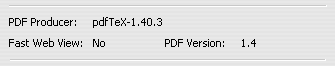
\includegraphics[width=0.54\textwidth]
		{pics/mark.png}
	\caption{Dokumen Dibuat dengan PDFLatex}
	\label{fig:pdflatex}
\end{figure}

Semoga template ini dapat membantu orang-orang yang ingin mencoba menggunakan 
\latex. Semoga template ini juga tidak berhenti disini dengan ada kontribusi 
dari para penggunanya. 
Kami juga ingin berterima kasih kepada Andreas Febrian, Lia Sadita, Fahrurrozi 
Rahman, Andre Tampubolon, dan Erik Dominikus atas kontribusinya dalam template 
ini. 

\vspace*{0.1cm}
\begin{flushright}
Depok, 30 Desember 2009\\[0.1cm]
\vspace*{1cm}
\penulis

\end{flushright}

\tableofcontents

\clearpage
\listoffigures
\clearpage
\listoftables
\clearpage

\addChapter{DAFTAR SINGKATAN}
\chapter*{DAFTAR SINGKATAN}

\addChapter{DAFTAR SIMBOL}
\chapter*{DAFTAR SIMBOL}

\addChapter{DAFTAR ISTILAH}
\chapter*{DAFTAR ISTILAH}

\addChapter{DAFTAR LAMPIRAN}
\chapter*{DAFTAR LAMPIRAN}

\pagenumbering{arabic}

%-----------------------------------------------------------------------------%
\chapter{\babSatu}
%-----------------------------------------------------------------------------%

%-----------------------------------------------------------------------------%
\section{Latar Belakang}
%-----------------------------------------------------------------------------%
Integrated Circuit (IC) merupakan modul teknologi dasar dari perangkat
elektronika tertanam modern. Dengan berkembangnya teknologi IC yang
mengutamakan ukuran kecil, dan performa yang tinggi serta dengan harga yang
murah membuat teknologi IC semakin diminati [1].

Dengan ukuran modul yang sangat kecil dan banyaknya komponen
pembangun, kerja sama antara desainer dilakukan untuk membangun sebuah
modul VLSI sehingga setiap desainer dapat fokus mendesain salah satu fungsi
yang terdapat dalam modul tersebut. Kerja sama dilakukan untuk mempermudah
pembuatan desain VLSI yang memiliki tingkat kerumitan yang tinggi. Desainer
juga dapat mempercepat waktu mendesain dengan menggunakan kode sumber
yang sudah ada atau bekerja sama secara paralel membuat masing-masing modul
yang nantinya akan digabung menjadi sebuah modul utama VLSI.

Setelah modul selesai dibuat maka modul siap untuk di-produksi. Dalam
proses produksi modul perusahaan tempat desainer bekerja tidak perlu memiliki
pabrik produksi modul sendiri, perusahaan dapat bekerja sama dengan mitra
percetakan yang akan memproduksi modul buatan perusahaan modul tersebut.
Cara kerja sama seperti ini disebut dengan Fabless Manufacturing [2]. Ketika
akan memproduksi IC, perusahaan harus menyerahkan blueprint modul VLSI ke
percetakan, namun blueprint tersebut tidak terjamin kerahasiaan nya serta
memungkinkan plagiarisme desain oleh oknum perusahaan atau pihak ketiga yang
tertarik menggunakan desain VLSI yang telah diserahkan untuk di-produksi.

Dengan memberikan rangkaian watermark sebagai pengamanan pada
blueprint VLSI siap cetak yang menandakan kepemilikan dari desainer atau
perusahaan produsen modul akan melindungi dari kecurangan pihak lain yang
akan mencuri desain. Sehingga kemungkinan pencurian atau plagiarisme yang
menyebabkan kerugian pada perusahaan atau desainer karena desain nya dicuri
atau di-plagiat berkurang

%-----------------------------------------------------------------------------%
\section{Rumusan Masalah}
%-----------------------------------------------------------------------------%
Berikut ini dijelaskan rumusan masalah yang dihadapi dalam proposal
penelitian Intelectual Property Protection (IPP) menggunakan metode Digital
Filter Algorithm using Logical Polymorph Gate Key Verification :

\begin{enumerate}
	\item Dengan metode Fabless Manufacturing, desain modul yang siap
	diproduksi diserahkan kepada perusahaan percetakan mitra sehingga
	mitra dapat mengetahui desain modul dari desainer yang
	memungkinkan desain dapat dicuri oleh oknum percetakan atau pihak
	ketiga yang tertarik dengan desain tersebut.
	 
	\item Desain modul rawan terhadap plagiarisme karena desain elektronik
	sangat mudah ditiru, sehingga pengamanan desain harus dilakukan agar
	desain tidak mudah untuk dicuri atau di-plagiat.
	
	\item Apabila pihak ketiga mencuri desain, desainer dapat mengklaim modul
	tersebut dengan bukti dari pengamanan watermark yang telah tertanam
	dalam IC menggunakan teknik pemanggilan watermark yang hanya
	diketahui oleh desainer yang mendesain IC tersebut.
\end{enumerate}
%-----------------------------------------------------------------------------%
\section{Tujuan}
%-----------------------------------------------------------------------------%
Berikut merupakan tujuan pengamanan desain modul yang siap cetak
sehingga aman terhadap pencurian hak cipta :
\begin{enumerate}
	\item Merancang rangkaian pengamanan dalam sebuah chip design sebagai
	bukti kepemilikan desain (ownership) atau watermarking.
	
	\item Desain chip yang telah diberi rangkaian watermark akan dianalisis
	perubahan performa dari desain sebelum dan sesudah watermarking
	serta kemungkinan watermark di-modifikasi oleh pihak lain atau
	reverse engineering untuk digunakan kembali oleh pengguna yang tidak
	sah.
	
	\item Rangkaian ini akan ditanam di dalam chip yang pemanggilan informasi
	pemilik dari chip hanya diketahui oleh pemilik cipta.
\end{enumerate}
%-----------------------------------------------------------------------------%
\section{Batasan Masalahan}
%-----------------------------------------------------------------------------%
Dalam penelitian ini rancangan desain VLSI yang disisipkan watermark
membatasi masalah serta pembahasan yang akan diteliti sebagai berikut :

\begin{enumerate}
	\item Tidak membuat modul IC VLSI spesifik, namun menggunakan yang
	sudah ada dan menyisipkan dengan watermark.
	
	\item Menyisipkan rangkaian dengan data watermark dan tidak membahas
	detail data dari pemilik cipta.
	
	\item Watermarking yang dilakukan untuk satu chip IC dan tidak mewatermark
	masing-masing modul yang ter-integrasi dalam chip IC. 
\end{enumerate}
%-----------------------------------------------------------------------------%
\section{Metodologi Penyelesaian Masalah}
%-----------------------------------------------------------------------------%
%\todo{Tuliskan metodologi penelitian yang digunakan.}

%-----------------------------------------------------------------------------%
\section{Sistematika Penulisan}
%-----------------------------------------------------------------------------%
Sistematika penulisan laporan adalah sebagai berikut:
\begin{itemize}
	\item Bab 1 \babSatu
	\item Bab 2 \babDua
	\item Bab 3 \babTiga
	\item Bab 4 \babEmpat
	\item Bab 5 \kesimpulan
\end{itemize}
%%%%%%%%%%%%%%%%%%%%%%%%%%%%%%%%%%%%%%%%%%%%%%%%%%%%%%%%%%%%
% 
%%%%%%%%%%%%%%%%%%%%%%%%%%%%%%%%%%%%%%%%%%%%%%%%%%%%%%%%%%%%

\chapter{\babDua}
Membuat desain sebuah perangkat IC membutuhkan proses yang panjang dan sumberdaya manusia yang banyak, serta tingkat ketelitian yang tinggi. Oleh karenanya di butuhkan biaya yang tidak kecil dan waktu yang cukup lama hanya untuk membuat sebuah desain IC. Dengan kerumitan yang tinggi serta waktu yang lama dalam setiap prosesnya kadang pihak yang tak bertanggung jawab melakukan kecurangna dengan mecuri desain untuk memotong waktu dan biaya yang di butuhkan utuk produksi. sehingga menjadi masalah dalam dunia permanufakturan ic. \cite{Azriel2017}

%%%%%%%%%%%%%%%%%%%%%%%%%%%%%%%%%%%%%%%%%%%%%%%%%%%%%%%%%%%%%
% 
%%%%%%%%%%%%%%%%%%%%%%%%%%%%%%%%%%%%%%%%%%%%%%%%%%%%%%%%%%%%%

\section{Very Large Scale Integration}
\textit{Very Large Scale Integration} atau disingkat VLSI merupakan proses pembuatan sebuah IC dengan mengkombinasikan ribuan transistor ke dalam sebuah \textit{chip}. VLSI ada sejak tahun 1970-an ketika semikonduktor kompleks dan teknologi komunikasi sedang berkembang. Mikroprosesor merupakan salah satu peraangkat VLSI. Sebelum adanya teknologi VLSI kebanyakan IC memiliki set fungsi yang terbatas yang dapat di jalankan. Sebuah perangkat chip elektronik dahulu hanya fokus pada sebuah fungsi seperti CPU, ROM, RAM dan rangkaian logika lainnya. Dengan adanya VLSI memungkinkan disainer IC untuk menambahkan berbagai fungsi kedalam sebuah chip IC. \cite{vlsi.hist} 

%%%%%%%%%%%%%%%%%%%%%%%%%%%%%%%%%%%%%%%%%%%%%%%%%%%%%%%%%%%%%
% 
%%%%%%%%%%%%%%%%%%%%%%%%%%%%%%%%%%%%%%%%%%%%%%%%%%%%%%%%%%%%%

\subsection{Arus Pengembangan LSI}
\textit{Integrated Circuit} (IC) merupakan teknologi sirkuit elektronika yang lebih maju. Sebuah rangkaian elektronika dibuat dari berbagai komponen elektronika yang berbeda beda seperti transistor, resistor, kapasitor dan dioda yang saling tersambung satu sama lain. \cite{vlsi.hist}

Transistor merupakan komponen terpenting pada pengembangan teknologi komputer moderen. Sebelum ditemukannya transistor. Para \textit{Engineer} harus menggunakan tabung vakum. Tabung vakum dapat bekerja sebagai saklar elektronik. Namun tabung vakum membutuhkan daya dan ruang yang besar, mahal, serta kemampuan eksekusi yang lambat membuat tabung vakum tergantikan oleh transistor.

Dengan ditemukannya transistor yang ukuran dan kebutuhan dayanya yang kecil namun tetap efektif, Para Engineer elektronik di tahun 1950an melihat banyak sekali kemungkinan untuk implementasinya pada rangkaian elektronik yang lebih maju. Dengan semakin meningkatnya kompleksitas pada rangkaian elektronik munculah masalah-masalah baru.

Salah satunya adalah ukuran rangkaian. Sebuah rangkaian kompleks seperti komputer sangat bergantung pada kecepatan. Apabila jumlah komponen pada komputer terlalu banyak maka sambungan antar komponen juga semakin banyak dan semakin panjang, sehingga menyebabkan kecepatan transfer sinyal listrik menjadi berkurang yang menyebabkan proses pada komputer menjadi lambat.

Tahun 1958 masalah ini dapat dipecahkan oleh ide \textit{Jack S Kilby} yang idenya adalah merangkai komponen elektronika dalam sebuah blok silikon (\textit{Monolithic Idea}). Idenya tersebut tidak hanya mengurangi ukuran rangkaian namun juga mengurangi kebutuhan kabel sambungan antar rangkaian serta manufakturingnya dapat diautomasi. Akan tetapi idenya tersebut masih memiliki banyak masalah lain. Walaupun begitu, idenya tersebut mendapatkan penghargaan nobel di tahun 2000.

Setengah tahun setelah \textit{Kilby} mencetuskan idenya tentang rangkaian \textit{Monolithic}. \textit{Robert Noyce} memiliki jawaban untuk beberapa permasalahan pada ide \textit{Kilby}. Yaitu interkoneksi antar rangkaian. Yaitu menambahkan lapisan metal pada lapisan terakhir dan menghilangkan sebagian lapisannya sehingga sambungan antar komponen dapat terbentuk.

\begin{figure}
	\centering
	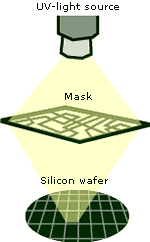
\includegraphics[width=0.35\textwidth]
	{pics/steping.png}
	\caption{Produksi Chip Moderen}
	\label{fig:produksiChipModeren}
\end{figure}

Chip pada zaman sekarang berbasis pada \textit{photolithography}. Pada teknik ini digunakan radiasi sinar \textit{Ultra Violet} yang melewati sebuah mask menuju lembaran silikon yang di lapisi filem \textit{photosensitive} untuk membentuk suatu rangkaian.

%%%%%%%%%%%%%%%%%%%%%%%%%%%%%%%%%%%%%%%%%%%%%%%%%%%%%%%%%%%%%
% 
%%%%%%%%%%%%%%%%%%%%%%%%%%%%%%%%%%%%%%%%%%%%%%%%%%%%%%%%%%%%%

\subsection{Kemungkinan Serangan Desain LSI}
Dilihat dari proses developing, terdapat 2 cara untuk mendapatkan sebuah desain untuk di kloning. Pertama dengan mengambil langsung data mentah desain atau "\textit{blueprint}" dan \textit{Reverse Engineering} saat barang telah dipublikasi di pasaran.

\begin{figure}
	\centering
	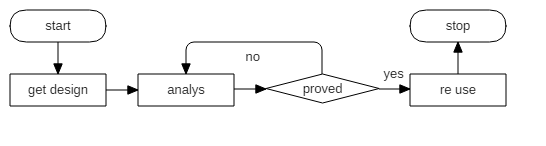
\includegraphics[width=1.05\textwidth]
	{diagrams/untrustSource.png}
	\caption{Clonning/Sumber Tidak Terpercaya}
	\label{fig:untrustsource}
\end{figure}

Dalam segi ini serangan dilakukan dengan cara mencuri langsung desain yang sudah siap di fabrikasi serta uji coba kebenaran. Bila pencuri mendapatkan desain yang telah di uji coba, maka pencuri tinggal langsung memperbanyak desain yang telah di curi.

\begin{figure}
	\centering
	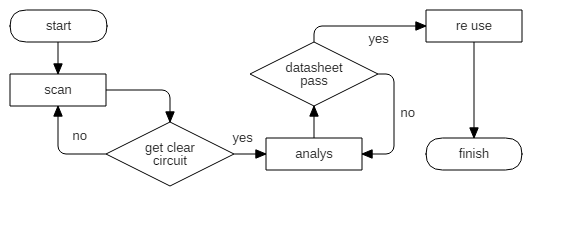
\includegraphics[width=1.05\textwidth]
	{diagrams/reverseEngineering.png}
	\caption{RE (Reverse Engineering)}
	\label{fig:reverseengineering}
\end{figure}

Untuk serangan jenis ini, pencuri sudah pendapatkan produk dari pasar yang telah teruji, pencuri tinggal melakukan scan rangkaian kemudian mengujinya dengan datasheet. Apabila hasil \textit{scan} desain produk di dapati rangkaian yang konkrit/jelas dan rangkaian tersebut telah teruji sesuai datasheet. Maka pencuri tinggal melakukan fabrikasi.

%%%%%%%%%%%%%%%%%%%%%%%%%%%%%%%%%%%%%%%%%%%%%%%%%%%%%%%%%%%%%
% 
%%%%%%%%%%%%%%%%%%%%%%%%%%%%%%%%%%%%%%%%%%%%%%%%%%%%%%%%%%%%%

\subsection{Mengatasi Serangan terhadap Desain LSI}
Dengan meninjau kemungkinan dari tipe serangan, terdapat berbagai cara untuk mengatasi setiap serangan serangan tersebut. Dari \textit{reverse engineering} hingga \textit{untrust source}. untuk \textit{reverse enginering} digunakan teknik \textit{anti reverse engineering} dan untuk \textit{untrust source} digunakan teknik \textit{identifier} dan dengan \textit{enclosure agreement law}.

\begin{figure}
	\centering
	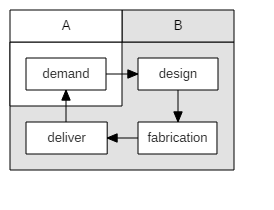
\includegraphics[width=0.5\textwidth]
	{diagrams/oldBusinessLSI.png}
	\caption{Model Bisnis Lama}
	\label{fig:oldbiss}
\end{figure}

Pada model gambar diatas, kegiatan desain, fabrikasi dan deliveri di lakukan oleh satu pihak yang sama. Proses pembuatan suatu perangkat IC dimonopoli oleh 1 perusahaan. Sehingga kemungkinan serangan hanya ada di antara pihak A dan Pihak B.

\begin{figure}
	\centering
	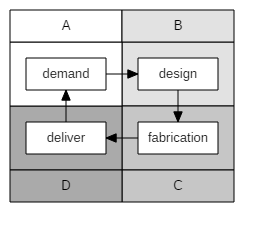
\includegraphics[width=0.5\textwidth]
	{diagrams/newBusinessLSI.png}
	\caption{Model Bisnis Baru}
	\label{fig:newbiss}
\end{figure}

Namun seiring dengan perkembangnya jaman. Monopoli proses dari desain, fabrikasi hingga \textit{deliveri} mulai sulit di terapkan. Karena dengan semakin berkembangnya zaman dan deman akan fitur desain semakin tinggi, otomatis biaya semakin tinggi dan kompleksitas suatu desain semakin rumit serta waktu untuk menyelesaikan suatu desain semakin lama.

Oleh karena itu sekarang mulai diterapkan \textit{Fabless manufacturing} atau \textit{joint venture} untuk membuat suat perangkat elektronika. Setidaknya pada proses bisnis ini terdapat 4 pihak. Pihak A dari keinginan pasar, pihak B yang melakukan perancangan desain, pihak C yang elakukan fabrikasi hasil rancangan pihak B dan Pihak D yang melakukan deliveri hasil fabrikasi di pihak C ke A.

%%%%%%%%%%%%%%%%%%%%%%%%%%%%%%%%%%%%%%%%%%%%%%%%%%%%%%%%%%%%%
% 
%%%%%%%%%%%%%%%%%%%%%%%%%%%%%%%%%%%%%%%%%%%%%%%%%%%%%%%%%%%%%

\section{Teknik Proteksi}
Dari berbagai teknik yang telah digunakan, penulis melakukan penggabungan 2 teknik pengamanan dalam sebuah desain IC. Dalam penelitian ini dilakukan penggabungan 2 teknik agar cakupan wilayah keamanan sebuah IC semakin luas. Berikut teknik yang digabungkan dalam penelitian kali ini.

\subsection{Digital Signal Processing Filter}
Digital Signal Prosesing (DSP) merupakan pengolahan sinyal digital, seperti digunakan pada komputer hingga untuk melakukan berbagai operasi proses sinyal. Sinyal yang diproses merupakan kumbulan bilangan sekuensial yang merepresentasikan sampel dari variabel sinyal kontinyu pada suatu domain seperti domain waktu, ruang atau frekuensi.

Pada pengolahan sinyal, sebuah filter adalah sebuah alat atau proses yang menghilangkan beberapa komponen atau fitur yang tidak di inginkan dari suatu sinyal. Filtering merupakan kelas proses sinyal.

\subsection{Polimorphisme Gate}
\textit{Polimorphisme Gate} merupakan teknik pengecoh yang di gunakan dalam perlindungan desain IC. Sebagai contoh sebuah rangkaian dengan \textit{output} F dan \textit{input} A,B dan C akan memiliki hasil yang berbeda jika parameters k yang diberikan berbeda. Misal bila parameter k diisi dengan kombinasi 0101 maka \textit{output}-nya adalah

\begin{equation}
	F = A XOR (A AND B)
\end{equation}
Sedangkan bila parameter k diisi dengan kombinasi 1101 maka outputnya menjadi

\begin{equation}
	F = A XOR (A \textbf{NOR} B)
\end{equation}

\begin{figure}
	\centering
	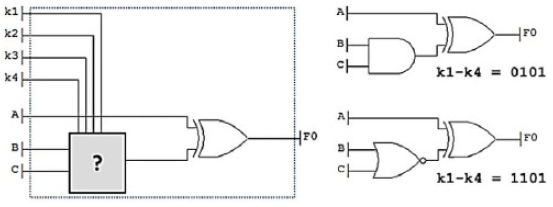
\includegraphics[width=0.75\textwidth]
	{pics/polymorphgate.png}
	\caption{Polymorph gate\cite{Chen2017a}}
	\label{fig:poly}
\end{figure}

%%%%%%%%%%%%%%%%%%%%%%%%%%%%%%%%%%%%%%%%%%%%%%%%%%%%%%%%%%%%%
% 
%%%%%%%%%%%%%%%%%%%%%%%%%%%%%%%%%%%%%%%%%%%%%%%%%%%%%%%%%%%%%

\section{Peralatan dan Teknologi}
Dalam penelitian kali ini dibutuhkan beberapa peralatan dan standard teknologi untuk mengembangkan teknik perlindungan intelektual properti. Sebagai penunjang dalam pembuatan perlindungan, penulis menggunakan tools dan teknologi yang umum digunakan dalam proses pengembangan desain LSI.

\subsection{Verilog HDL}
\textit{Verilog HDL} merupakan bahasa pendeskripsi hardware yang digunakan untuk mendesain dan dokumentasi sistem elektronika. Verilog HDL memungkinkan perancang mendesain pada berbagai tingkatan abstraksi.

\textit{Verilog HDL} berasal dari \textit{Automated Integrated Design System} (yang kemudian berubah nama menjadi \textit{Gateway Design Automation}) pada tahun 1985. Saat itu perusahaan tersebut dipegang oleh Dr. Prabhu Goel, pendiri \textit{PODEM test generation algorithm}. \textit{Verilog HDL} di desain oleh Phil Moorby, yang kemudian menjadi \textit{chief Designer} untuk \textit{Verilog-XL} dan perusahaan rekan pertama di \textit{Cadance Design System}. 

Awalnya \textit{Verilog} dibuat sebagai bahasa simulasi. Kemudian setelah berkembang tidak hanya digunakan untuk simulasi namun juga untuk sintesis. (source www.verilog.com)

\subsection{Yosys Open SYnthesis Suite}
\textit{Yosys} adalah sebuah framework untuk sintesis \textit{Verilog RTL}. Sekarang ini memiliki suport yang extensif pada \textit{Verilog-2005} dan mendukun berbagai set basik algoritme sintesis untuk berbagai domain aplikasi.

\begin{figure}
	\centering
	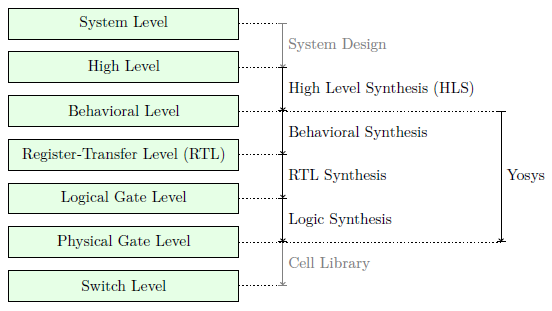
\includegraphics[width=0.75\textwidth]
	{pics/yosys.png}
	\caption{Perbedaan Tinkatan Abstraksi dan Sintesis Yosys\cite{link.yosys}}
	\label{yosys}
\end{figure}

\subsection{Xilinx ISE Design Suit}
\textit{Xilinx ISE Design Suit} merupakan \textit{Computer Aided Design} (CAD) keluaran \textit{Xilinx} yang digunakan untuk \textit{developing} IC.

\begin{figure}
	\centering
	
\includegraphics[width=0.4\textwidth]
	{pics/ise-logo.jpg}
	\caption{Logo Xilinx ISE Design Suit\cite{link.logo}}
	\label{ise}
\end{figure}

\subsection{FPGA Elbert V2 Board}
FPGA merupakan kepanjangan dari \textit{Field Programmable Gate Array} adalah perangkat keras yang biasa digunakan dalam proses manufakturing IC. FPGA digunakan untuk mensimulasikan draft rancangan IC yang siap untuk di test yang apabila telah lolos test akan di lanjutkan ke tahap \textit{layout}. FPGA hanya digunakan apabila rancangan membutuhkan input dari perangkat lain atau program kernel.

\begin{figure}
	\centering
	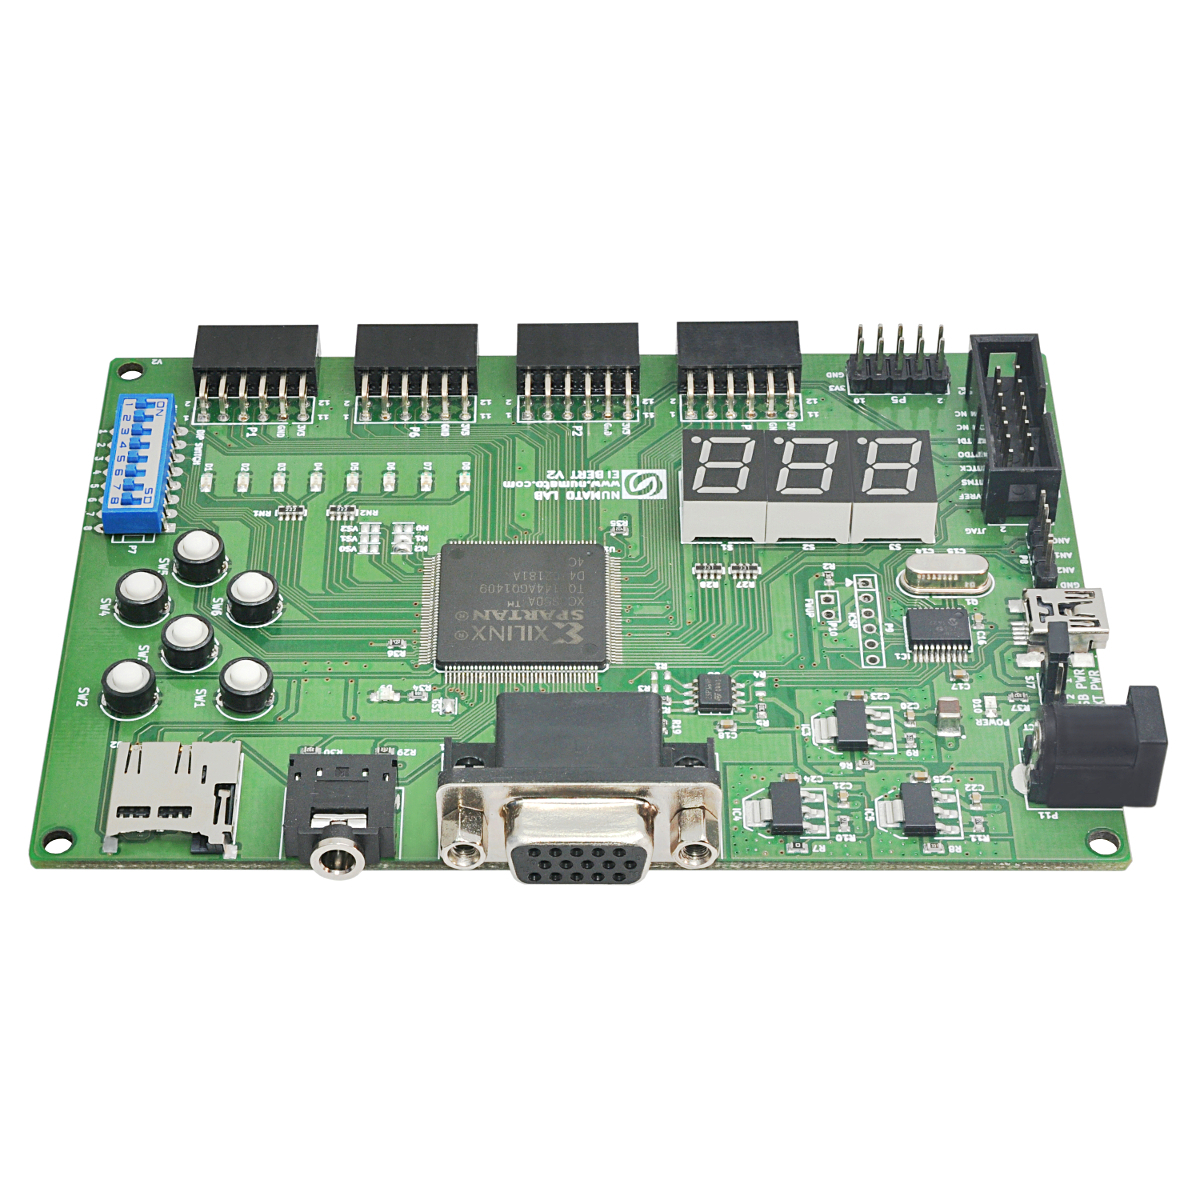
\includegraphics[width=0.75\textwidth]
	{pics/elbertv2.jpg}
	\caption{FPGA Board - Elbert V2\cite{link.board}}
	\label{fig:fpga}
\end{figure}

\textit{Elbert V2} merupakan \textit{Board} yang simpel namun serbaguna untuk pembelajaran atau pengembangan. \textit{Board} ini menggunakan \textit{Xilinx Spartan 3A FPGA}. Pada \textit{Development Board} ini memiliki fitur \textit{FPGA} dari \textit{Xilinx XC3S50A} dengan 144 pin dengan maksimum 108 user IO. Dilengkapi dengan antarmuka \textit{USB2} untuk kemudahan konfigurasi ke \textit{SPI flash}. 

%%%%%%%%%%%%%%%%%%%%%%%%%%%%%%%%%%%%%%%%%%%%%%%%%%%%%%%%%%%%%
% 
%%%%%%%%%%%%%%%%%%%%%%%%%%%%%%%%%%%%%%%%%%%%%%%%%%%%%%%%%%%%%

\section{Target IP Core}
Watermark adalah rangkaian yang tidak boleh berdiri sendiri pada implementasinya walaupun dalam pengembangannya bisa di lakukan mandiri. Dalam penelitian kali ini Modul yang akan di watermark adalah modul ALU.

\subsection{Aritmatic Logic Unit (ALU)}
\textit{Aritmatik Logic Unit} (ALU) adalah kombinasi rangkaian elektronik digital yang melakukan fungsi aritmatika dan operasi bitwise pada bilangan integer binari. Ini sangat kontras dengan Floating Point Unit (FPU), yang melakukan operasi bilangan floating point. Sebuah ALU pada dasarnya bagian dari berbagai macam blok rangkaian komputasi, termasuk Central Prosesing Unit (CPU). Sebuah CPU, FPU, atau GPU mungkin memiliki banyak ALU di dalamnya.

\begin{figure}
	\centering
	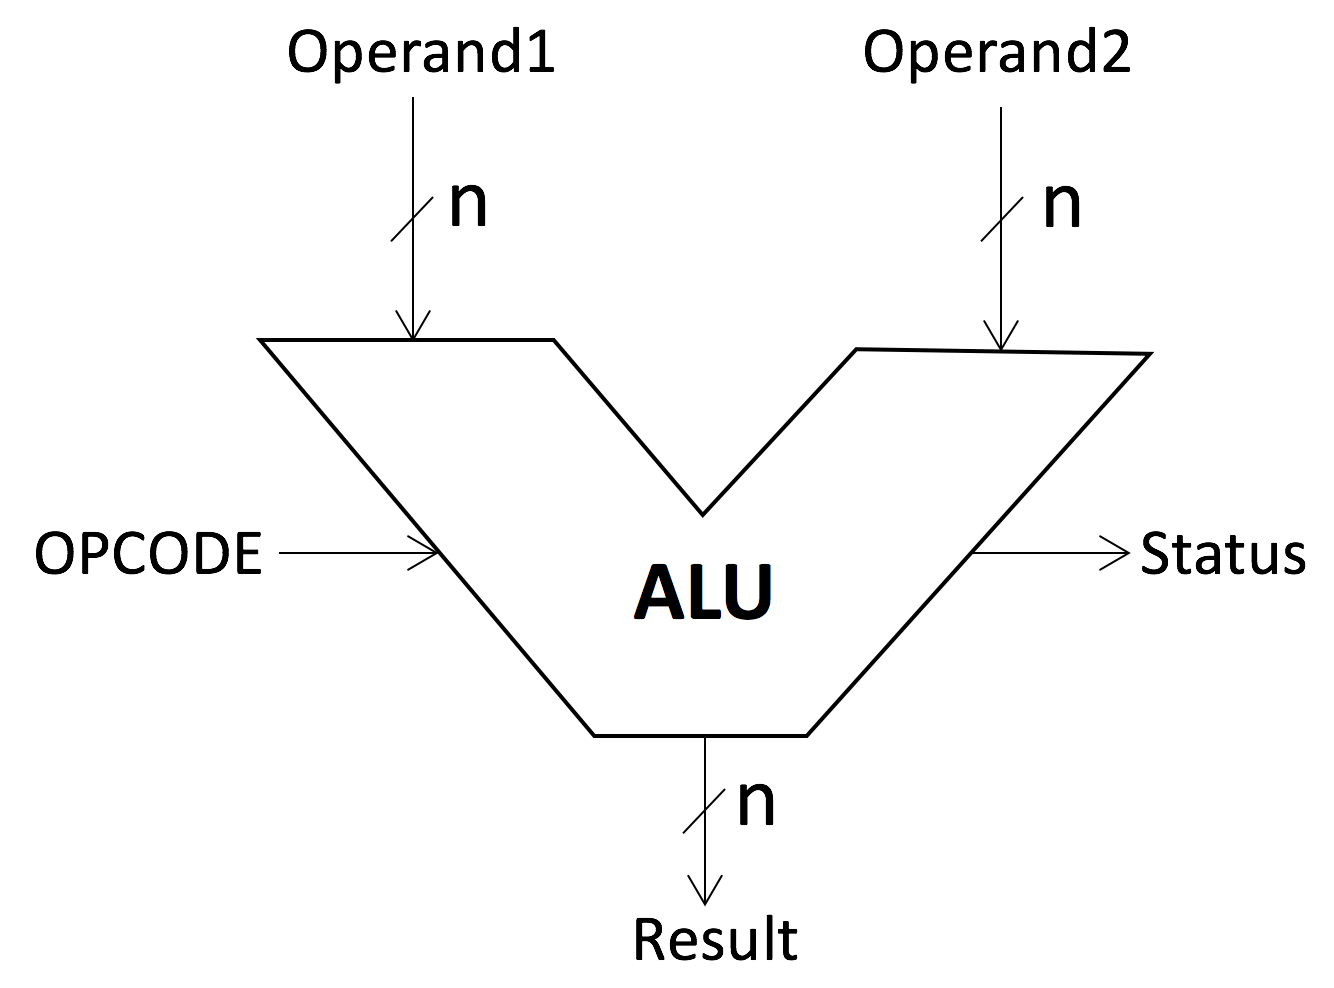
\includegraphics[width=0.5\textwidth]
	{pics/alu.png}
	\caption{ALU}
	\label{alu}
\end{figure}


%-----------------------------------------------------------------------------%
\chapter{\babTiga}
%-----------------------------------------------------------------------------%
\todo{tambahkan kata-kata pengantar bab 1 disini}


%-----------------------------------------------------------------------------%
\section{Satu Persamaan}
%-----------------------------------------------------------------------------%

\noindent \begin{align}\label{eq:garis}
	\cfrac{y - y_{1}}{y_{2} - y_{1}} = 
	\cfrac{x - x_{1}}{x_{2} - x_{1}}
\end{align}

\equ~\ref{eq:garis} diatas adalah persamaan garis. 
\equ~\ref{eq:garis} dan \ref{eq:bola} sama-sama dibuat dengan perintah \bslash
align. 
Perintah ini juga dapat digunakan untuk menulis lebih dari satu persamaan. 

\noindent \begin{align}\label{eq:bola}
	\underbrace{|\overline{ab}|}_{\text{pada bola $|\overline{ab}| = r$}} 
		= \sqrt[2]{(x_{b} - x_{a})^{2} + (y_{b} - y_{a})^{2} + 
				\vert\vert(z_{b} - z_{a})^{2}}
\end{align}

%-----------------------------------------------------------------------------%
\section{Lebih dari Satu Persamaan}
\label{sec:multiEqu}
%-----------------------------------------------------------------------------%
\noindent \begin{align}\label{eq:matriks}	
	|\overline{a} * \overline{b}| &= |\overline{a}| |\overline{b}| \sin\theta 
		\\[0.2cm]
	\overline{a} * \overline{b} &=  
		\begin{array}{| c c c |}
			\hat{i} & x_{1} & x_{2} \\
			\hat{j} & y_{1} & y_{2} \\
			\hat{k} & z_{1} & z_{2} \\
		\end{array} \nonumber \\[0.2cm]
	&= \hat{i} \,
		\begin{array}{ | c c | }
			y_{1} & y_{2} \\
			z_{1} & z_{2} \\
		\end{array} 
	   + \hat{j} \,
		\begin{array}{ | c c | }
			z_{1} & z_{2} \\
			x_{1} & x_{2} \\
		\end{array} 
	   + \hat{k} \,	
		\begin{array}{ | c c | }
			x_{1} & x_{2} \\
			y_{1} & y_{2} \\
		\end{array}
		\nonumber
\end{align}

Pada \equ~\ref{eq:matriks} dapat dilihat beberapa baris menjadi satu bagian 
dari \equ~\ref{eq:matriks}. 
Sedangkan dibawah ini dapat dilihat bahwa dengan cara yang sama, \equ~
\ref{eq:gabungan1}, \ref{eq:gabungan2}, dan \ref{eq:gabungan3} memiliki nomor 
persamaannya masing-masing. 

\noindent \begin{align}\label{eq:gabungan1}	
	\int_{a}^{b} f(x)\, dx + \int_{b}^{c} f(x) \, dx = \int_{a}^{c} f(x) \, dx
		\\\label{eq:gabungan2}
	\lim_{x \to \infty} \frac{f(x)}{g(x)} = 0 \hspace{1cm} 
		\text{jika pangkat $f(x)$ $<$ pangkat $g(x)$} \\\label{eq:gabungan3}
	a^{m^{a \, ^{n}\log b }} = b^{\frac{m}{n}}
\end{align}


%-----------------------------------------------------------------------------%
\chapter{\babEmpat}
%-----------------------------------------------------------------------------%
\todo{tambahkan kata-kata pengantar bab 1 disini}
% Table generated by Excel2LaTeX from sheet 'Daya'
\begin{table}[htbp]
	\centering
	\caption{Add caption}
	\begin{tabular}{|l|c|c|c|}
		\hline
		\multicolumn{1}{|c|}{Desain} & Total & Dinamic & Static \bigstrut\\
		\hline
		Original & 10.42 & 00.00 & 10.42 \bigstrut\\
		\hline
		original Watermark & 11.47 & 01.05 & 10.42 \bigstrut\\
		\hline
		Selisih & 01.05 & 01.05 & 00.00 \bigstrut\\
		\hline
		equivalen & 9,19\% & 100,00\% & 0,00\% \bigstrut\\
		\hline
	\end{tabular}%
	\label{tab:addlabel}%
\end{table}%


% Table generated by Excel2LaTeX from sheet 'Data io'
\begin{table}[htbp]
	\centering
	\caption{Add caption}
	\begin{tabular}{|c|c|c|c|cccc}
		\cline{1-4}\cline{6-8}    \multirow{2}[4]{*}{Time} & \multicolumn{3}{c|}{in} & \multicolumn{1}{c|}{} & \multicolumn{3}{c|}{out} \bigstrut\\
		\cline{2-4}\cline{6-8}          & 0     & 1     & 2     & \multicolumn{1}{c|}{} & \multicolumn{1}{c|}{0} & \multicolumn{1}{c|}{1} & \multicolumn{1}{c|}{2} \bigstrut\\
		\cline{1-4}\cline{6-8}    0     & 1     & 1     & 1     & \multicolumn{1}{c|}{} & \multicolumn{1}{c|}{0} & \multicolumn{1}{c|}{0} & \multicolumn{1}{c|}{0} \bigstrut\\
		\cline{1-4}\cline{6-8}    1     & 1     & 0     & 1     & \multicolumn{1}{c|}{} & \multicolumn{1}{c|}{0} & \multicolumn{1}{c|}{1} & \multicolumn{1}{c|}{0} \bigstrut\\
		\cline{1-4}\cline{6-8}    2     & 1     & 1     & 0     & \multicolumn{1}{c|}{} & \multicolumn{1}{c|}{0} & \multicolumn{1}{c|}{0} & \multicolumn{1}{c|}{0} \bigstrut\\
		\cline{1-4}\cline{6-8}    3     & 0     & 1     & 0     & \multicolumn{1}{c|}{} & \multicolumn{1}{c|}{0} & \multicolumn{1}{c|}{0} & \multicolumn{1}{c|}{1} \bigstrut\\
		\cline{1-4}\cline{6-8}    4     & 0     & 1     & 1     & \multicolumn{1}{c|}{} & \multicolumn{1}{c|}{0} & \multicolumn{1}{c|}{1} & \multicolumn{1}{c|}{1} \bigstrut\\
		\cline{1-4}\cline{6-8}    5     & 1     & 0     & 0     &       &       &       &  \bigstrut\\
		\cline{1-4}    6     & 0     & 1     & 0     &       &       &       &  \bigstrut\\
		\cline{1-4}    7     & 0     & 0     & 0     &       &       &       &  \bigstrut\\
		\cline{1-4}    8     & 1     & 1     & 1     &       &       &       &  \bigstrut\\
		\cline{1-4}    9     & 1     & 0     & 0     &       &       &       &  \bigstrut\\
		\cline{1-4}    10    & 0     & 1     & 0     &       &       &       &  \bigstrut\\
		\cline{1-4}    11    & 0     & 0     & 1     &       &       &       &  \bigstrut\\
		\cline{1-4}    12    & 0     & 1     & 0     &       &       &       &  \bigstrut\\
		\cline{1-4}    13    & 1     & 0     & 1     &       &       &       &  \bigstrut\\
		\cline{1-4}    14    & 0     & 1     & 1     &       &       &       &  \bigstrut\\
		\cline{1-4}    15    & 1     & 0     & 0     &       &       &       &  \bigstrut\\
		\cline{1-4}    16    & 0     & 1     & 0     &       &       &       &  \bigstrut\\
		\cline{1-4}    17    & 1     & 1     & 1     &       &       &       &  \bigstrut\\
		\cline{1-4}    18    & 0     & 1     & 1     &       &       &       &  \bigstrut\\
		\cline{1-4}    19    & 0     & 0     & 0     &       &       &       &  \bigstrut\\
		\cline{1-4}    \end{tabular}%
	\label{tab:addlabel}%
\end{table}%


%---------------------------------------------------------------
\chapter{\kesimpulan}
%---------------------------------------------------------------
\todo{Tambahkan kesimpulan dan saran terkait dengan perkerjaan 
	yang dilakukan.}


%---------------------------------------------------------------
\section{Kesimpulan}
%---------------------------------------------------------------


%---------------------------------------------------------------
\section{Saran}
%---------------------------------------------------------------


%
% Daftar Pustaka 
% 

% 
% Tambahkan pustaka yang digunakan setelah perintah berikut. 
% 
\begin{thebibliography}{4}

\bibitem{latex.intro}
{Jeff Clark. (n.d). \f{Introduction to LaTeX}.
26 Januari 2010. \url{http://frodo.elon.edu/tutorial/tutorial/node3.html}.}

\bibitem{chapman}
R. Chapman and T. S. Durrani, “IP Protection of DSP Algorithms for System on Chip Implementation,” vol. 48, no. 3, pp. 854–861, 2000.

\bibitem{water}
“Watermarking Techniques for Electronic Circuit Design,” no. 1, pp. 1–17.

\bibitem{lui}
Q. Liu, W. Ji, Q. Chen, and T. Mak, “IP Protection of Mesh NoCs Using Square Spiral Routing,” vol. 24, no. 4, pp. 1560–1573, 2016.

\bibitem{cui}
A. Cui, C. Chang, S. Member, S. Tahar, and S. Member, “A Robust FSM Watermarking Scheme for IP Protection of Sequential Circuit Design,” vol. 30, no. 5, pp. 678–690, 2011.

\bibitem{nie}
T. Nie, “Performance Evaluation for IP Protection Watermarking Techniques.”

\bibitem{zhang1}
J. Zhang, Y. Lin, Y. Lyu, G. Qu, and S. Member, “A PUF-FSM Binding Scheme for FPGA IP Protection and Pay-Per-Device Licensing,” vol. 10, no. 6, pp. 1137–1150, 2015.

\bibitem{zhang2}
J. Zhang, Y. Lin, Q. Wu, and W. Che, “Watermarking FPGA Bitfile for Intellectual Property Protection,” pp. 764–771.

\bibitem{kahng}
A. B. Kahng et al., “Watermarking Techniques for Intellectual Property Protection.”

\bibitem{mosh}
V. G. Moshnyaga and H. Nita, “STG-based Detection of Power Virus Inputs in FSM.”

\end{thebibliography}



\begin{appendix}
	%
% @author  Andreas Febrian
% @version 1.00 
% 
% Hanya sebuah pembatas bertuliskan LAMPIRAN ditengah halaman. 
% 

\begin{titlepage}
	\centering 
	\vspace*{6cm}
	\noindent \Huge{LAMPIRAN}
	\addChapter{LAMPIRAN}
\end{titlepage}
	\setcounter{page}{2}
	%-----------------------------------------------------------------------------%
\addChapter{Lampiran 1}
\chapter*{Lampiran 1}
%-----------------------------------------------------------------------------%
\end{appendix}

\end{document}